\chapter{Navigation and Cohabitation for Co-located Users in Limited Workspace}
\label{chapter:navigation}
\minitoc

\section{Introduction}
Navigation is one of the most important and fundamental interaction that we have within the virtual environment.

\section{Virtual Navigation}

\subsection{Definition}
A lot of navigation techniques of different nature exist to allow users to travel through large virtual space, while physically stay within a limited workspace. These navigation techniques can be classified according to the control law - how a given input from the user can be mapped to a position or velocity change in the virtual world. Typical control laws include position and rate control, and can be implemented by both hardware and software solutions.

\subsection{Taxonomy}
The most studied position control is natural walking, which is considered to be the most intuitive way to explore the virtual environment \citep{Ruddle2009BW}. To enable infinite walking in restricted real workspace, one can use both physical locomotion devices like treadmills \citep{Iwata1999Treadmill} and software solutions (e.g. redirection \citep{Peck2008RED}, resetting \citep{Williams2007ELV} and scaling techniques \cite{Interrante2007SLB}). Besides natural walking, walk-in-place \citep{Razzaque2002RWP} and WIM (World-In-Miniature) \citep{Stoakley1995VRW} are also interesting alternatives. Moreover, \citet{Fleury2010Generic} proposed a general model to integrate physical workspace into the virtual world and make the user aware of the physical environment in different ways. \citet{Cirio2012Cube} also summarized several metaphors for safe navigation in a restricted cubic workspace.

Conversely to previous techniques, rate control techniques are based on a virtual vehicle model which enables navigation in large virtual scenes. Users control directly the vehicle's velocity instead of position in the virtual world and can have the sensation of moving (self-motion illusion or vection \citep{Riecke2012Vection}). Actually the virtual vehicle can be controlled by information coming from different sources, for example, various input devices like joystick, haptic arm \citep{Martin2012Forklift} or even specific locomotion devices \citep{Marchal2011JOYMAN}. With video cameras or optical tracking systems, users can specify the velocity of the vehicle by motion tracking data of the hand (camera-in-hand \citep{Ware1990EVC}) or head movements \citep{Bourdot2002HCNav}. Gestures \citep{Konrad2003Gesture} and postures \citep{Kapri2011Steering} can also be used to move the virtual vehicle. Bowman et al. named this kind of virtual navigation techniques steering metaphors \citep{Bowman2004UIT} which are often relatively easy to implement and can provide efficient and flexible control of virtual navigation.

Some navigation metaphors such as the bubble technique \citep{Dominjon2005Bubble} and the magic barrier tape \citep{Cirio2009MBT} combine both position and rate control in order to enable infinite navigation within restricted real workspace. Position control is used within the physical workspace and then rate control is applied to the virtual vehicle to move further in the virtual world.

\subsection{Evaluation}
It's not obvious to compare different navigation techniques without a given virtual context and the associated task. Nevertheless, \citet{Bowman1997TIV} have proposed a list of quality factors which can help us to compare and measure the performance of navigation techniques including general performance indicators such as velocity and accuracy, spatial awareness, ease of learning, ease of use, and level of presence. General performance indicators are relatively easy to measure. We can choose factors that we need depending on the given task and the configuration of the virtual scene.

The level of presence is an important factor for the use of navigation techniques in an immersive virtual environment. \citet{Slater1994DepthPre} consider presence as a subjective phenomenon that can be defined as the sensation of being in a virtual environment, while \citet{Witmer1998MPV} relate presence in part to the concept of attention. These authors believe that both involvement and immersion are necessary for experiencing presence. \citet{Schuemie2001Pres} have proposed a taxonomy of different measures of presence and a detailed analysis of factors that influence presence in the virtual environment.

Another important factor is the user comfort, particularly symptoms related to cybersickness. \citet{Rich1996AICS} have examined the relationship between the user's level of control of his/her own movements and cybersickness, while \citet{So2001ENS} have carried out experiments to study the influence of the navigation speed (both linear and circular components) on the level of severity of cybersickness. A study by \citet{Stanney2002HPIVE} gives us a better global view that addresses different perceptive factors that are susceptible to cause cybersickness. \citet{LaViola2000DCV} has also discussed about the physiological aspects and theories of cybersickness. To evaluate the level of cybersickness, the Simulator Sickness Questionnaire (SSQ) \citep{Kennedy1993SSQ} remains the reference tool despite the development of various physiological measurements.

\subsection{Summary}


\section{Addressed Issues}
\subsection{Navigation in Limited Workspace}
It is essential to keep user's safety when immersed in the virtual world. The navigation technique should prevent users from reaching the limits of the physical workspace. Some navigation metaphors such as the bubble technique \citep{Dominjon2005Bubble} and the magic barrier tape \citep{Cirio2009MBT} combine both walking and vehicle-based control in order to enable infinite navigation within restricted real workspace. \citet{Cirio2012Cube} summarized several metaphors for safe navigation in a restricted cubic workspace. Moreover, \citet{Fleury2010Generic} proposed a general model to integrate physical workspace into the virtual world and make the user aware of the physical environment in different ways.

\subsection{User Cohabitation}
Immersive virtual environment has the power to bring users to an artificial world by blocking the perception of the real world. In such situation users often forget boundaries of the physical workspace due to visual immersion, which could endanger both the user and the device. For some devices with non-closed display such as large image wall or a 3-wall CAVE, immersion is limited to the display area.

The human joystick metaphor does not necessarily prevent users from running into physical obstacles or keep user's field of view within projected areas. Moreover, if multiple users share the same immersive device for co-located collaboration with each one using a human joystick metaphor, they may have user cohabitation problems: users may run into collision when they move around without paying attention to other users (Figure~\ref{fig:3_illustration} left); one can also disrupt the visual perception of the virtual world of another if the former appears to be in the field of view of that user due to body occlusion (Figure~\ref{fig:3_illustration} right).

\begin{figure*}[tb]
  \centering
  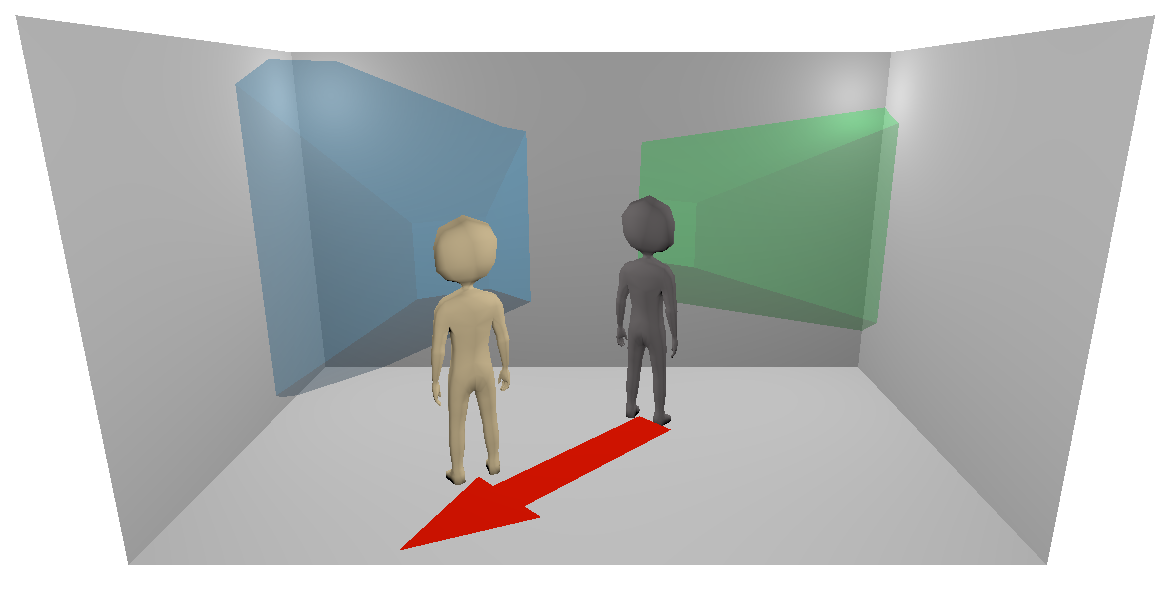
\includegraphics[width=0.49\textwidth]{figures/ch3/illu_col}
  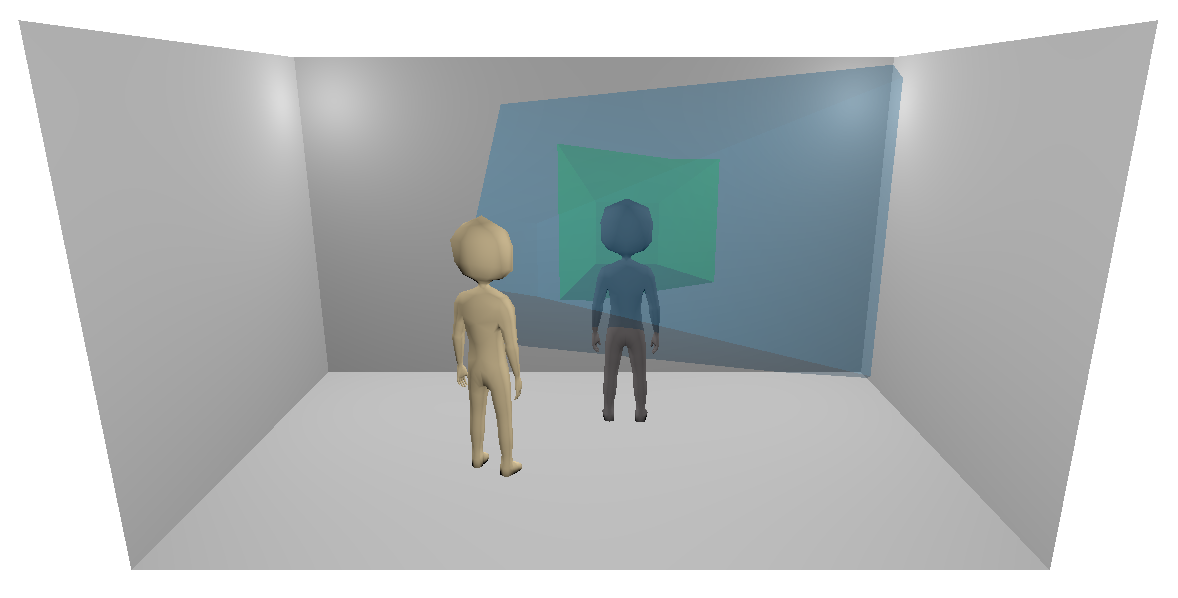
\includegraphics[width=0.49\textwidth]{figures/ch3/illu_occ}
  \caption{\label{fig:3_illustration}Illustration of collision (left) and occlusion (right) between co-located users in a multi-stereoscopic 3-wall plus floor CAVE.}
\end{figure*}

So to support safe and functional free navigation in an immersive context, the original human joystick metaphor should be adapted according to the number of co-located users and the configuration of the immersive system (size and shape of the screen walls, effective tracking space, etc.).

Two aspects of the problem should be solved: how to manage the spatial relationship between active users and the immersive display boundaries, i.e. how to prevent users from touching the wall screens and from seeing non projected areas, and how to provide enough workspace for each co-located user and thus avoid collision and occlusion between them.

When it comes to managing multiple users in the same immersive virtual environment for co-located collaboration, most works focused only on closely coupled collaboration (e.g. co-manipulation). In this case, virtual navigation is either disabled or controlled by a leader and shared by other users \citep{Beck2013IGG, Kulik2011CSS}. To enable more complex collaborative scenarios including loosely coupled tasks which require individual navigation for co-located users, we should propose novel navigation models that comply with user cohabitation constrains.

\subsection{Summary}

\section{Approach - Altered Human Joystick}

\subsection{Basic Model}
The basic navigation method we use is a reduced version (from 6DoF to 3DoF) of a head-controlled navigation technique (Figure~\ref{fig:3_hcnav}) proposed by \citet{Bourdot2002HCNav}. It is actually a human joystick metaphor \citep{McMahan2012EDF}, but with an additional degree of freedom for yaw rotation. User's head position and orientation are captured in real time with an optical tracker attached to the 3D glasses.

To navigate, user first needs to choose a neutral reference frame (composed of a position and an orientation ($P_{0}, \theta_{0}$)) during calibration. Then user can move in the real workspace relatively to this reference frame to control the linear and angular velocity of the vehicle ($\overrightarrow{v_{veh}}, \Omega_{veh}$), denoting $(P, \theta)$ the current configuration. The translation and rotation gain functions are configured respectively by coefficients $K_{T}$ and $K_{R}$.

\begin{equation}
\overrightarrow{v_{veh}}=K_{T}\cdot \overrightarrow{P_{0}P}
\end{equation}
\begin{equation}
\overrightarrow{\Omega_{veh}}=K_{R}\cdot \widehat{\theta_{0}\theta}
\end{equation}

\begin{figure}[tb]
  \centering
  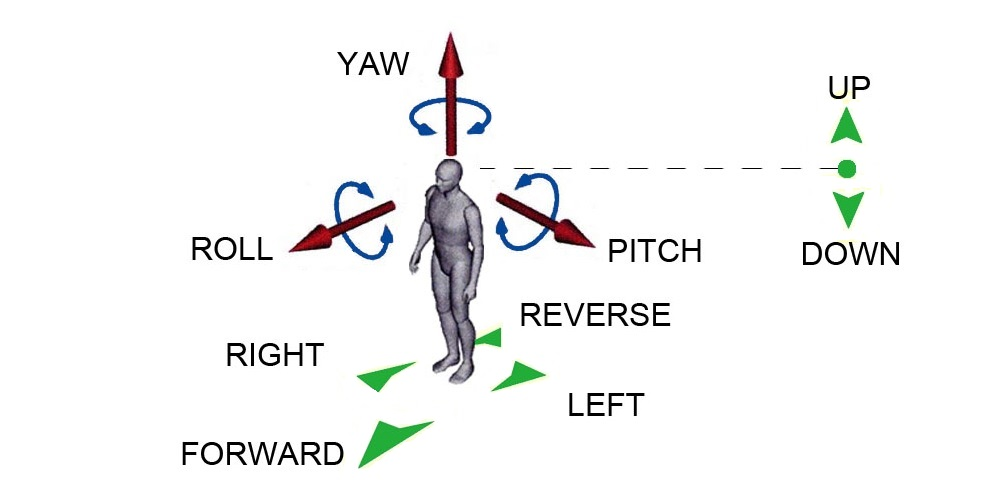
\includegraphics[width=0.8\textwidth]{figures/ch3/HCNav}
  \caption{\label{fig:3_hcnav}Head-controlled navigation paradigm.}
\end{figure}

\subsection{Alterations}

\subsubsection{Altered Gain Function}
 To restrain user's translational workspace, we can replace the linear gain function with a divergent one integrating the distance limitation into the navigation model.

\begin{equation}
\overrightarrow{v_{veh}}=K_{T}\cdot \left(\frac{\Delta x}{X_{m}-\Delta x},\:\frac{\Delta y}{X_{m}-\Delta y}\right)
\end{equation}

where $X_{m}$ is the minimum distance from the neutral position $P_{0}$ to the border of the physical system (Figure~\ref{fig:3_workspace_border}a). This divergent gain function allows user to apply an infinite vehicle velocity when reaching $X_{m}$. So the workspace of a user is defined by the physical space that user is free to move inside before reaching any borders.

\begin{figure}[tb]
\begin{center}
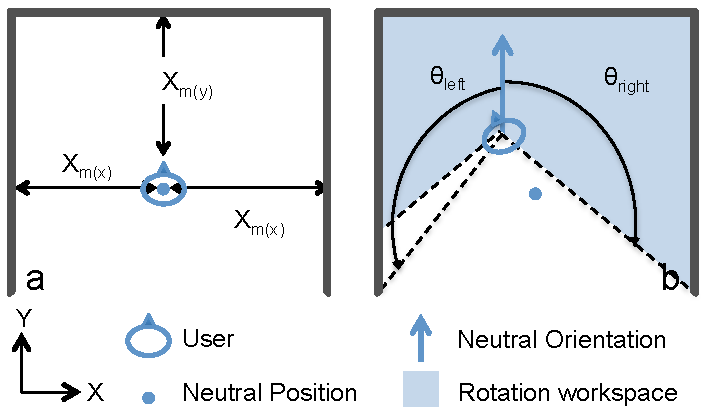
\includegraphics[width=0.6\textwidth]{figures/ch3/workspace_border}
\par\end{center}
\caption{\label{fig:3_workspace_border}(a) The maximum available workspace $X_{m}$ can have different values on x and y axis. (b) User's rotational workspace is defined by $\theta_{max}$ on both sides of the neutral orientation.}
\end{figure}

To avoid collision between users, we can consider each user as a moving border which restricts directly the workspace of other users. However, this method makes the velocity control too unstable when all users move the same time. A possible compromised solution is to assign each user a safe zone for proper use, and an overlapped zone to share with others. We adjust the ``virtual border" of one user's workspace depending on the penetration of other users in the shared area. This way a user's velocity will only be influenced by others when he/she is inside the shared zone, one can make use of the entire shared zone as if he/she was alone in the system until the other user also needs to use it. Figure~\ref{fig:3_adaptive_trans_border} shows an example of two users inside a 3-wall CAVE system. Usually CAVE-like systems are in a rectangular form, so the border formed by a user is chosen to be a vertical plane.

\begin{figure}[tb]
\begin{center}
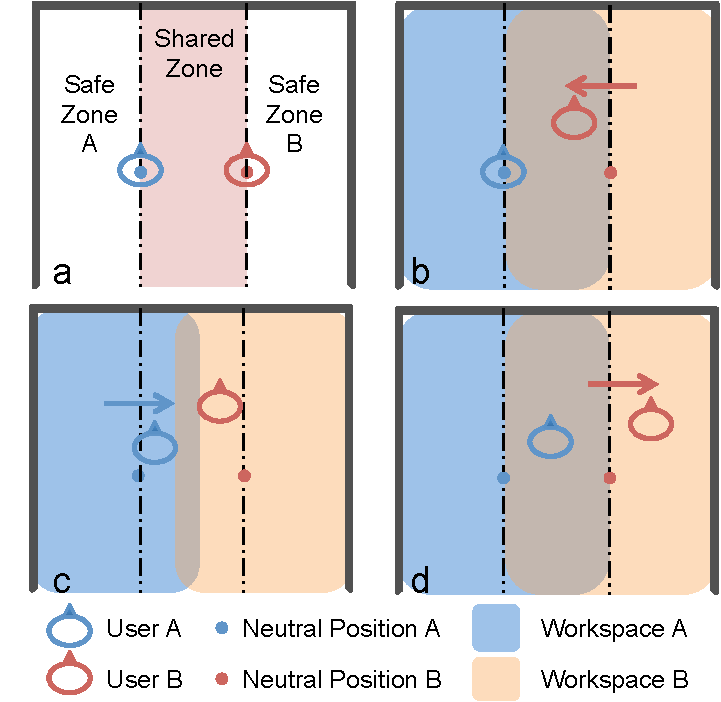
\includegraphics[width=0.6\textwidth]{figures/ch3/adaptive_trans_border}
\end{center}
\caption{\label{fig:3_adaptive_trans_border}Adaptive border of user's workspace for translation in a two-user case : a) Initial state. b) User B moves into the shared zone while user A is still in the safe zone, both users' workspaces are not influenced and user B can use the entire shared zone. c) User A also moves into the shared zone and pushes the border of user B's workspace to the right. d) User B moves back to the safe zone, the entire shared zone can now be used by user A.}
\end{figure}

Considering rotations, physical constrains could also be integrated into the gain function similarly as for translation. For example, in a 3-wall CAVE it is preferable to avoid user occlusions and prevent users from seeing the empty screen behind them. However, due to the different nature between translation and rotation movements, we chose to use a saturated quadratic gain function rather than a divergent form as follows:

\begin{equation}
\Omega_{veh}=
  \begin{cases}
    \frac{\Omega_{max}}{(\theta_{max})^{2}}\cdot(|\Delta\theta|)^{2} & \text{if } |\Delta\theta|<\theta_{max} \\
    \Omega_{max} & \text{if } |\Delta\theta| \geq \theta_{max}
  \end{cases}
\end{equation}

where $\theta_{max}$ represents the maximum available rotational workspace (with which the user reaches the maximum rotation speed $\Omega_{max}=\pi\, rad.s^{-1}$) computed as the minimum of $\theta_{left}$, $\theta_{right}$ and $\theta_{user}$ to provide a symmetric vehicle control around the neutral orientation $\theta_{0}$ (Figure~\ref{fig:3_workspace_border}b).  


\subsubsection{Adaptive Neutral Reference Frame}

The original human joystick metaphor has a fixed neutral reference frame (a neutral position and orientation) defined during calibration. This reference frame should give user the maximum workspace that the physical working environment can offer, for example, the center of a CAVE is often a good choice. However, when we have mobile obstacles in the physical working environment, e.g. multiple co-located users, it may be inappropriate to have a fixed reference frame. With the above methods of computing user's available workspace, a fixed neutral reference frame distribution will often lead to non-symmetric use of the total available workspace both for translation and rotation.

To optimize workspace usage, we can reconfigure each user's neutral reference frame as the center of his/her available workspace (Figure~\ref{fig:3_neutral_ref}). In this way, each user's workspace is balanced between constrains introduced by the display system and by other users, and is always symmetric on the left and right with respect to the neutral reference frame.

Although this method could make better use of the total workspace, it also potentially increases the mutual influence between users, which may be disturbing for the navigation control. When users have relatively small workspace, the variation of neutral reference frame may remain imperceptible during navigation, which is to be tested.   

\begin{figure}[tb]
  \centering
  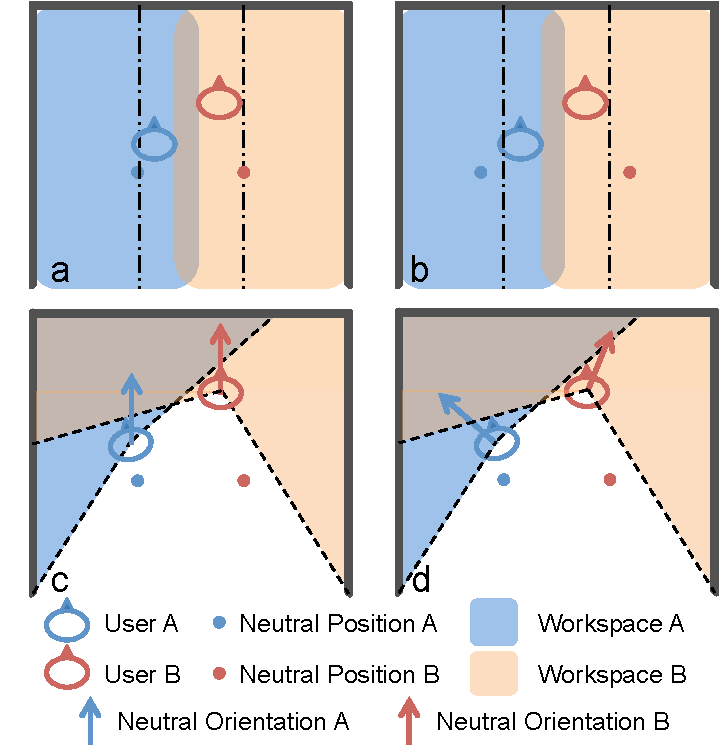
\includegraphics[width=0.6\textwidth]{figures/ch3/neutral_ref}
  \caption{\label{fig:3_neutral_ref}(a, c) Users' neutral reference frames are fixed to the initial distribution. (b, d) Users' neutral reference frames are computed dynamically according to both users' positions.}
\end{figure}

\subsection{Combinations}
With the two categories of alterations presented above, we can create a set of similar navigation methods by combining these modifications. To see more clearly the impacts of each modification, we created three groups of navigation methods (see table~\ref{tab:3_combinations}). In the first two groups (Group T and Group R), we deactivated respectively rotation and translation, and we kept both for the last group (Group TR). For Group R, since users are not supposed to change their positions, the neutral orientations will always be fixed, though they will be different depending on how they are computed (be facing the front screen or be the bissectrice of rotational workspace).

\begin{table*}[!t]
\renewcommand{\arraystretch}{1.3}
\caption{A List of Altered Versions of Human Joystick divided in Three Groups}
\label{tab:3_combinations}
\centering
\begin{tabular}{c l p{2.5cm} l p{2.5cm}}
  \hline
  Technique & \multicolumn{2}{c}{Translation} & \multicolumn{2}{c}{Rotation} \\
   & Form & Neutral Position & Form & Neutral Orientation \\ \hline
  T1 & Linear & Fixed & / & / \\
  T2 & Linear & Adaptive & / & / \\
  T3 & Divergent & Fixed & / & / \\
  T4 & Divergent & Adaptive & / & / \\ \hline
  R1 & / & / & Linear & Face front screen \\
  R2 & / & / & Linear & Bissectrice \\
  R3 & / & / & Saturated Quadratic & Face front screen \\
  R4 & / & / & Saturated Quadratic & Bissectrice \\ \hline
  TR1 & Linear & Fixed & Linear & Fixed \\ TR2 & Linear & Fixed & Linear & Adaptive \\
  TR3 & Linear & Adaptive & Linear & Fixed \\ TR4 & Linear & Adaptive & Linear & Adaptive \\
  TR5 & Divergent & Fixed & Saturated Quadratic & Fixed \\ TR6 & Divergent & Fixed & Saturated Quadratic & Adaptive \\
  TR7 & Divergent & Adaptive & Saturated Quadratic & Fixed \\ TR8 & Divergent & Adaptive & Saturated Quadratic & Adaptive \\
  \hline
\end{tabular}
\end{table*}

\subsection{Summary}

\section{Evaluations}
\subsection{Introduction}
In this paper, we extend the existing cohabitation model by adding additional alterations. Then we present three refined experiments to have an exhaustive analysis of different combinations of these alterations respectively in translation-only, rotation-only and translation-rotation combined navigation conditions. In this way we can see more clearly the impact of each alteration and the interaction between them.

\subsection{Measures}
We are interested in information coming from two different sources: how well they could achieve goals and manage navigation in the virtual world, and how they position themselves with respect to the screens and other users in the physical workspace. Some information could be collected directly or indirectly through logs, others could only for now be gathered via questionnaires. Here we summarized three categories of measurements that we used for evaluation.

\subsubsection{Navigation Performance Metrics}
For a pure navigation task, measurements like task finishing time (or speed) and trajectory length are often used to evaluate user's navigation efficiency.

\subsubsection{User Cohabitation Capacity Metrics}
User cohabitation concerns both users' spatial relationship with the limitation of physical system and disturbance between users. We propose an evaluation model containing four variables covering all these aspects to measure user cohabitation capacity in a restricted physical workspace.

When several autonomous entities move within a restricted physical workspace, whether they will have cohabitation problem depends not only on where they are, but also on the moment when they have spatial coincidence. So all these variables combine spatial and temporal dimensions, and higher scores suggest higher disturbance level.

\paragraph{\textbf{Hazardous Area Consumption}}
In the real world, we choose to define an ``Hazardous area" including all positions closer than $D_{Hazard}=1$ meter to any physical obstacle as shown on Figure \ref{fig:3_metrics}a.

In this area, user's presence and safety may be in balance depending both on the user real speed $\overrightarrow{v_{real}}$ which may affect collision probability, and on his/her relative distance to the screens $d_{screen[i]}$. So we compute a relative score $V_{hac}$ based on $\overrightarrow{v_{real}}$ and $d_{screen[i]}$ when the user is inside the hazardous area. 

\begin{equation}
S = 
  \begin{cases}
  \overrightarrow{v_{real}}\cdot\overrightarrow{n_{i}} & \text{if } \overrightarrow{v_{real}}\cdot\overrightarrow{n_{i}} \leq 0 \\
  0 & \text{if } \overrightarrow{v_{real}}\cdot\overrightarrow{n_{i}} > 0
  \end{cases}
\end{equation}

\begin{equation}
V_{hac}=\sum_{t_{initial}}^{t_{final}}\left(\sum_{i=1}^{i=3}\left(\frac{S}{d_{screen[i]}}\right)\right)
\end{equation}
where $\overrightarrow{n_{i}}$ is the screen's normal vector.


\paragraph{\textbf{Shared Workspace Occupation}}
In a two-user case, they share part of their translation workspace. To estimate the probability of user collision in the shared zone, we measure each user's penetration distance in the shared workspace $\Delta P_{sh}(t)=\left|(\overrightarrow{P}-\overrightarrow{P_{0}}).\overrightarrow{x}\right|$ while the other user is also inside the shared area (cf. Figure \ref{fig:3_metrics}b), and $\Delta P_{sh}(t)=0$ otherwise.

\begin{figure}[tb]
  \centering
  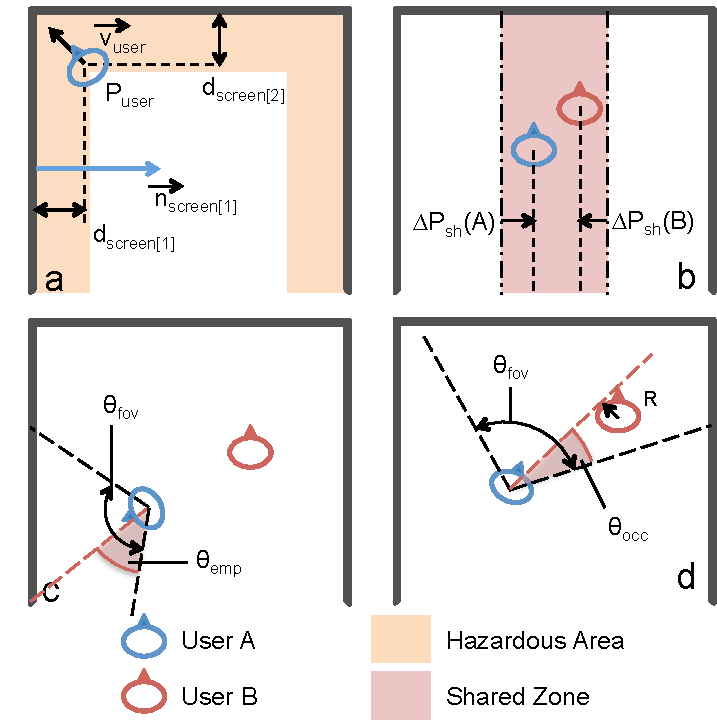
\includegraphics[width=0.6\textwidth]{figures/ch3/cohab_metrics}
  \caption{\label{fig:3_metrics}(a) The hazardous area. (b) User's penetration $\Delta P_{sh}(t)$ in the shared zone. (c) Illustration of seeing empty screen angle $\theta_{emp}(t)$ and (d) the occlusion angle $\theta_{occ}(t)$.}
\end{figure}

Using this penetration information, we can define a variable $V_{Psh}$ allowing to evaluate users' shared area usage taking in account both amplitude and duration of each user's usage situation as:

\begin{equation}
V_{Psh}=\int_{t_{init}}^{t_{final}}\Delta P_{sh}(t)\cdot dt
\end{equation}

\paragraph{\textbf{Empty Screen Perception}}
We define a variable $V_{emp}$ to evaluate to what extent and how long a user sees the empty screen behind by using $\theta_{emp}(t)$ (Figure \ref{fig:3_metrics}c)

\begin{equation}
V_{emp}=\int_{t_{init}}^{t_{final}}\theta_{emp}(t)\cdot dt
\end{equation}

\paragraph{\textbf{User Occlusion}}
In order to evaluate the occlusion phenomenon, we define a penalty angle $\theta_{occ}(t)$ which quantifies the non-usable part of the field of view where the perception of other users disrupts the perception of the virtual world as shown on Figure \ref{fig:3_metrics}d. This angle can be expressed, using the current user position $P$, the head orientation $\overrightarrow{H}$, the total available field of view $\theta_{fov}$ , the other user position $P'$ and a bounding cylinder radius $R$ which represented the size of the disturbing user, as:

\begin{equation}
\theta_{occ}=\frac{\theta_{fov}}{2}-\widehat{(\overrightarrow{H,}\overrightarrow{PP'})}+arcsin(\frac{R}{\left\Vert \overrightarrow{PP'}\right\Vert })\mathrm{\:,\: with\:}\theta_{occ}\geq0
\end{equation}

Using this occlusion angle, we define a variable $V_{occ}$ which allows to evaluate the importance of the occlusion problem considering both occlusion amplitude and duration computed as:

\begin{equation}
V_{occ}=\int_{t_{init}}^{t_{final}}\theta_{occ}(t)\cdot dt
\end{equation}


\subsubsection{Subjective Questionnaires}
Questionnaires are very useful tools to get user's subjective feelings (like presence and cybersickness) and explanations of certain choices and behaviors.

In our experiments, since we compared similar navigation conditions with minor differences, the level of presence was not our primary concern. However, these alterations could be source of cybersickness, so we used the Simulator Sickness Questionnaire (SSQ) \cite{Kennedy1993SSQ} to assess user's level of cybersickness before and after each test. In addition, we developed a light-weight cohabitation questionnaire to further investigate user's feeling towards disturbances coming from physical surroundings as well as from the other user (see Appendix~\ref{appendix:cohab_q}).

\subsection{Pre-test Condition}
In all the experiments below we tested the cohabitation of two users. The initial distribution of both users' neutral reference frames was defined as follows: each user's neutral position had equal distance to the nearest obstacle on the left and right, and they were moved 0.6m away from the front screen to leave more space for user to move forward. The neutral orientations were chosen to be face the front screen (Figure~\ref{fig:3_initial_config}). At the beginning of each task trial, users were always situated at the neutral position and facing the neutral orientation.

\begin{figure}[tb]
  \centering
  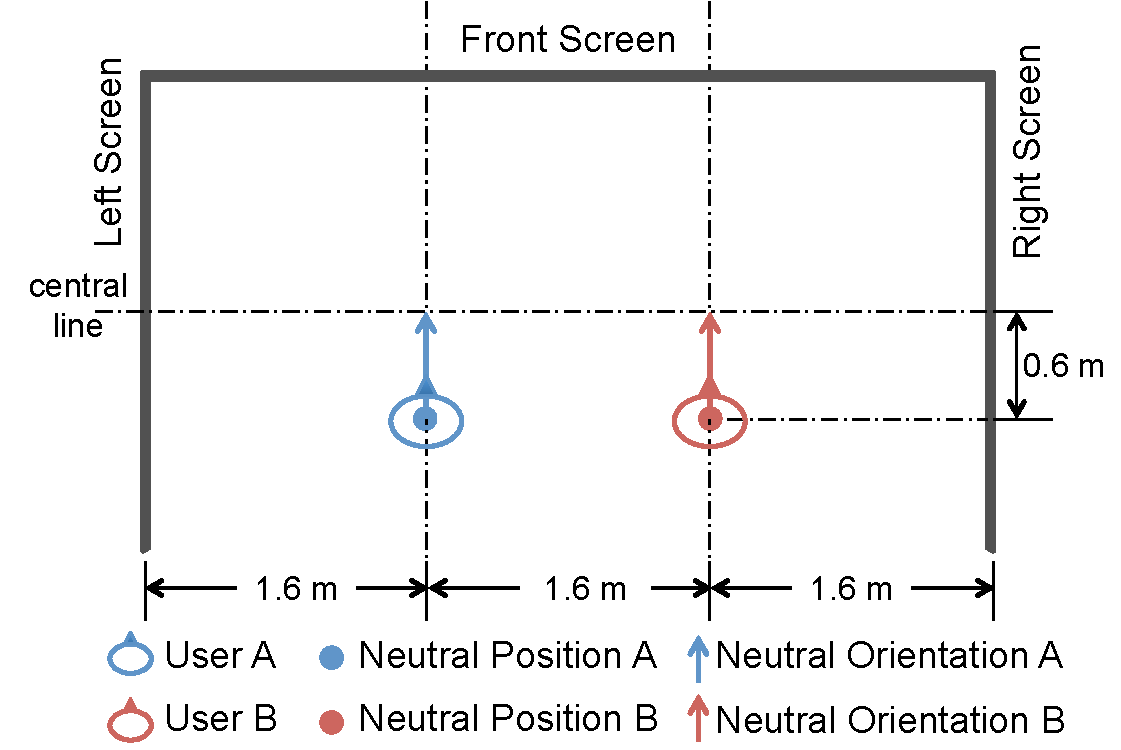
\includegraphics[width=0.8\textwidth]{figures/ch3/initial_config}
  \caption{\label{fig:3_initial_config}The initial distribution of users' neutral reference frames in our CAVE platform.}
\end{figure}

Before passing real tests, participants had a training session during which they spent about three to five minutes in a virtual playground to get familiar with the original human joystick metaphor.

\subsection{Collaborative Case Study}
\subsubsection{Design}
We conducted a first user study \citep{Chen2015Cohab} with 36 participants divided into pairs to test modified gain functions in a two-user working scenario. We defined three test conditions:

\begin{itemize}
  \item \textbf{C1}: Original human joystick with linear gain functions for translation and rotation (served as control condition).
  \item \textbf{C2}: Human joystick technique with modified gain functions.
  \item \textbf{C3}: C2 plus adaptive neutral orientation.
\end{itemize}

Back then, the idea of adaptive neutral reference frame was not fully developed and we were not sure whether that would be beneficial, so we formed C3 in addition to C2 as a beta test of reorientation of the neutral reference frames (their positions remained fixed).

We assumed that modified gain functions (C2) would improve users' cohabitation capacity, thus improve their navigation performance compared to linear gain functions (C1). We also assumed that as adaptive neutral orientation provided better distribution of user's rotational workspace, users should have less occlusion with C3 than C2.

Participants were invited to accomplish an object-finding task inside a virtual factory (Figure~\ref{fig:3_teaser_exp1}). The factory had five similar sections each containing a common working zone and two storage areas connected by corridors. The task was for each participant to bring target objects from different storage areas to the common working zone. Since the task was relatively complicated (based on a realistic working scenario) and had a pre and post questionnaire session (for the evaluation of cybersickness), we used an between-subject design with each pair of participants testing one of the three conditions.

\begin{figure}[tb]
  \centering
  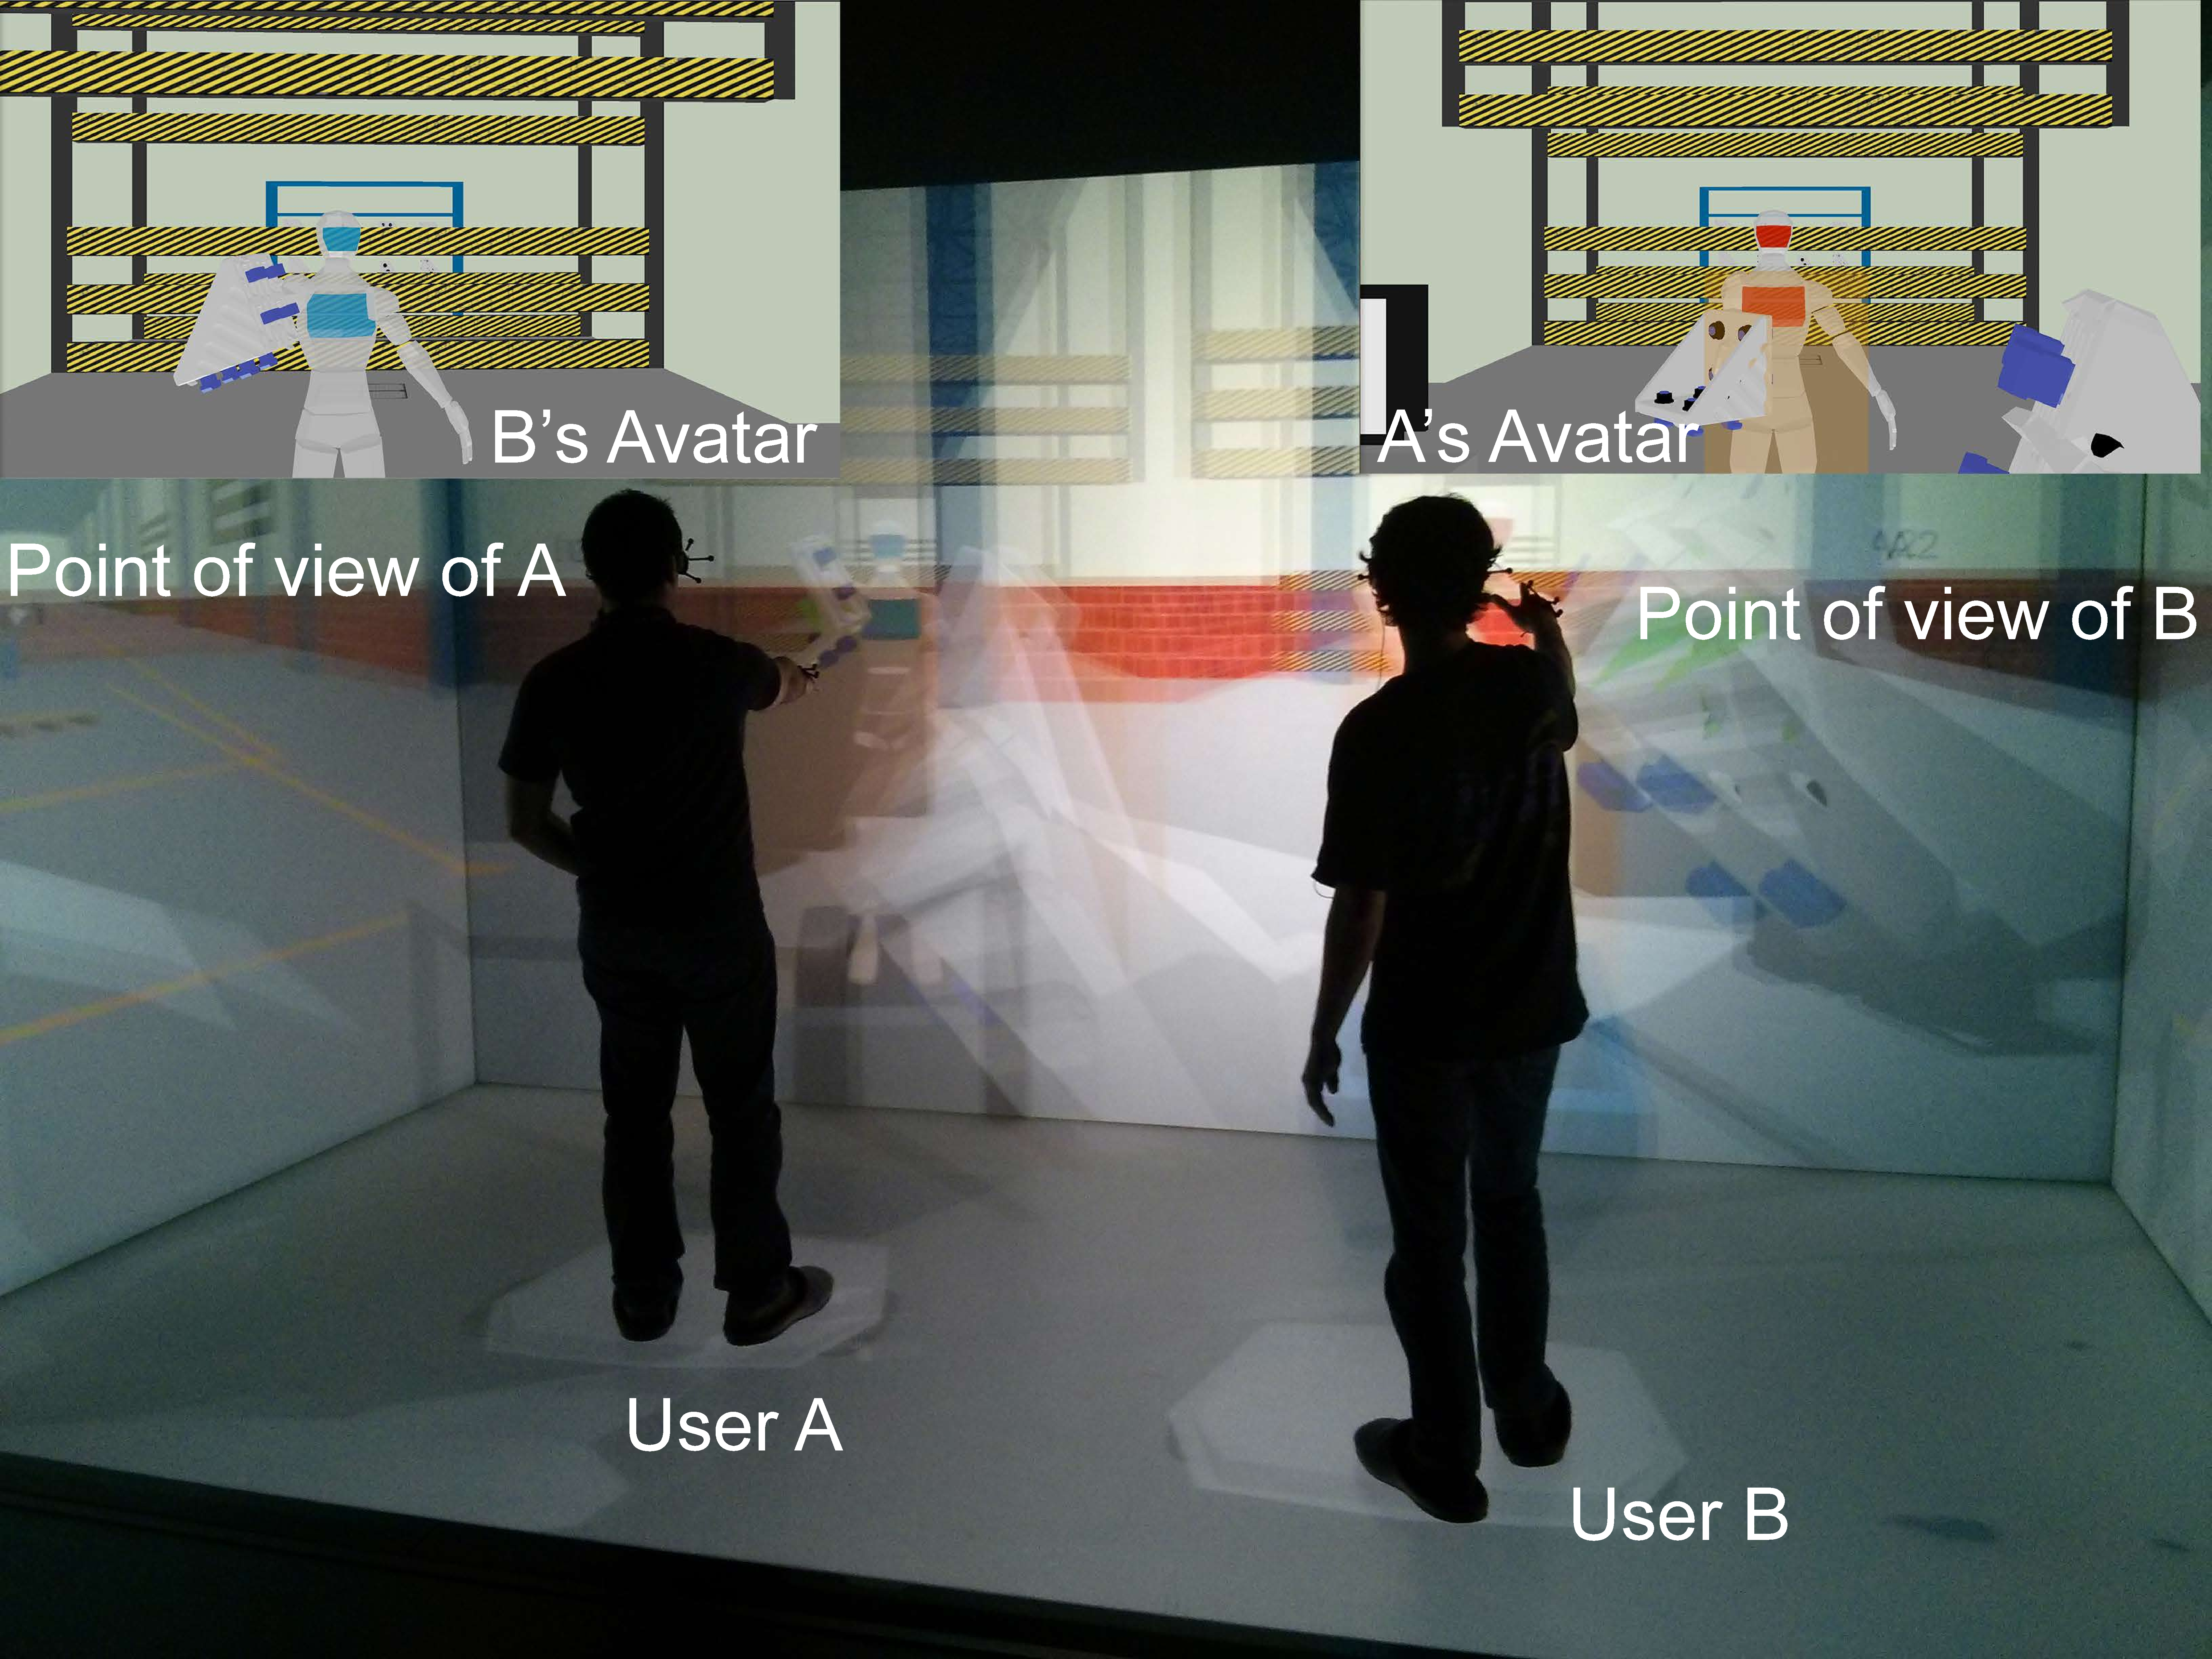
\includegraphics[width=0.8\textwidth]{figures/ch3/teaser_exp1}
  \caption{\label{fig:3_teaser_exp1}Two users worked inside a multi-stereoscopic CAVE system to finish an object-finding task. They were virtually face to face to put down collected objects.}
\end{figure}

\subsubsection{Results}
To summarize, participants had similar navigation performance both in terms of speed and precision under different conditions. And for user cohabitation capacity, main effects were found on Shared Workspace Occupation ($V_{Psh}$) (H(2, N=36) = 6.109610, p=0.047) with C3 (mean=1.402, sd=0.921) less than C2 (mean=2.826, sd=1.431), and on Occlusion Angle ($V_{occ}$) (H(2, N=36) = 21.08269, p\textless{} 0.0001) with C3 (mean=14.7, sd=31.0) less than C1 (mean=153.4, sd=71.4) and C2 (mean=90.3, sd=84.9).

Participants under all three conditions experienced mild cybersickness symptoms (Total score: C1: mean=15.58, sd=20.41; C2: mean=18.39, sd=19.37; C3: mean=13.4, sd=10.51), however, no significant difference were found between these conditions.

\subsubsection{Discussion}
The lack of significant difference between C1 and C2 could be explained by several observations. First, during navigation tasks, users were not necessarily synchronized with each other and were free to choose their navigation speed and trajectory. Regarding navigation control, they also had the choice between yaw rotation and lateral displacements, combined with forward movement to achieve the same virtual trajectory. Therefore it was difficult to predict users' real world movements and the recorded data had a large subject-dependent variation. Second, users were generally more cautious and conservative than we expected. They rarely went too close to the screen or to the other user to get high navigation speed by fear of running through virtual walls or barrels, which lessened cohabitation problems. The average navigation velocity measured under the three conditions were similar (around 2 m/s), which meant that the divergent part of C2 and C3 were seldom reached by users with the given gain values.

Finally, C3 was proved to have better support for reducing user occlusion. The way we defined the neutral orientations provided symmetric rotational workspace for users and tended to maintain an open angle between neutral orientations. In addition, we observed that C3 was also the best technique to minimize the occupation of the shared workspace (cf. $V_{Psh}$). Actually, as the neutral orientation defined user's main walking axis, the adaptive neutral orientations allowed more frequent use of safe zones rather than the shared zone in the middle.

Although we did not find significant results to prove the benefits of modified gain functions as we assumed in this experiment, important lessons were learned for future study of user cohabitation in a multi-stereoscopic immersive system. First of all, for a given task inside an immersive device with fixed size, a properly chosen gain value can reduce the chance for having user cohabitation problems even with linear gain function. In other words, to show the limitations of linear gain functions, we should use smaller gain value. Second, it was difficult to distinguish the influence of each individual modification due to the divergence in users' navigation strategies. To tackle that, we could test translation and rotation under separate conditions (Group T and Group R) as presented in Table~\ref{tab:3_combinations}. At last, we found it beneficial to have adaptive neutral orientation, which led us to extend the alterations by setting the neutral position $P_{0}$ of each user dynamically to see if we can get similar benefits as performing neutral orientation change. So besides C1, C2 and C3, which corresponded respectively TR1, TR5 and TR6 (Table~\ref{tab:3_combinations}), we made a complete list of eight conditions to test all possible combinations.

Moreover, the alterations tested in this experiment did not seem to provoke more symptoms of cybersickness, which made it viable for us to extend the model and conduct more refined experiments.

\subsection{Refined Experiments}
We conducted three additional experiments to complete previous user study. As explained above, we globally lowered the base gain value for all gain functions. In Experiment T (Translation only) and Experiment R (Rotation only), we created two special groups of navigation conditions by cutting off respectively rotation and translation, while in Experiment TR (Translation with Rotation) we kept both. All the three groups of conditions were listed in table \ref{tab:3_combinations} and to be tested with different types of navigation tasks. 

We compared these conditions in terms of navigation performance and cohabitation capacity to see the influence of each alteration and the effect of their combinations. What's different from previous user study was that participants were equipped with closed headphones to avoid perceiving the other user by audio cues (foot steps, verbal communications, etc.) since the alterations of the navigation metaphor only provided visual feedback.

Based on the results of previous experiment, we did not measure the level of cybersickness this time because of the number and similarity of test conditions. Instead, we used a light-weight questionnaire in Experiment TR (Appendix~\ref{appendix:cohab_q}) to get additional information on user cohabitation.

For all the experiments below, we performed one-way ANOVA test to compare different variables as within-subject factors. For post-hoc analyses, we used TukeyHSD multiple comparisons of means. All the analyses were performed with R\footnote{http://www.r-project.org/}. The results presented in this section were considered statistically significant when p \textless{} 0.05. Results having a p value between 0.05 and 0.1 were also presented as a trend effect.

\subsubsection{Participants}
12 participants (11 male, 1 female), aged from 24 to 54 (mean=32) were involved in our user study. They were divided into six pairs and each pair passed successively Experiment T, R and TR.

\subsubsection{Experiment T}
\paragraph{Design}
To compare the four navigation techniques in the first group (T1 - T4), we asked participants to accomplish a navigation task several times with each time a different technique. Thus, each navigation technique was tested once and the four conditions were randomized for different groups of participants.

The task was to travel to the other side of a straight corridor by following a given path marked by a white line on the floor and crossing all the gates along the path (Figure~\ref{fig:3_task1}). Each pair of participants had parallel corridors with symmetric path to walk through so they have more chance to collide in the physical workspace. To begin, participants left their departure areas and traveled to destination zones on the other side of the corridors. Once both participants arrived, they were teleported to the departure areas to begin the next round with a different navigation technique till all the conditions were tested.

\begin{figure}[tb]
  \centering
  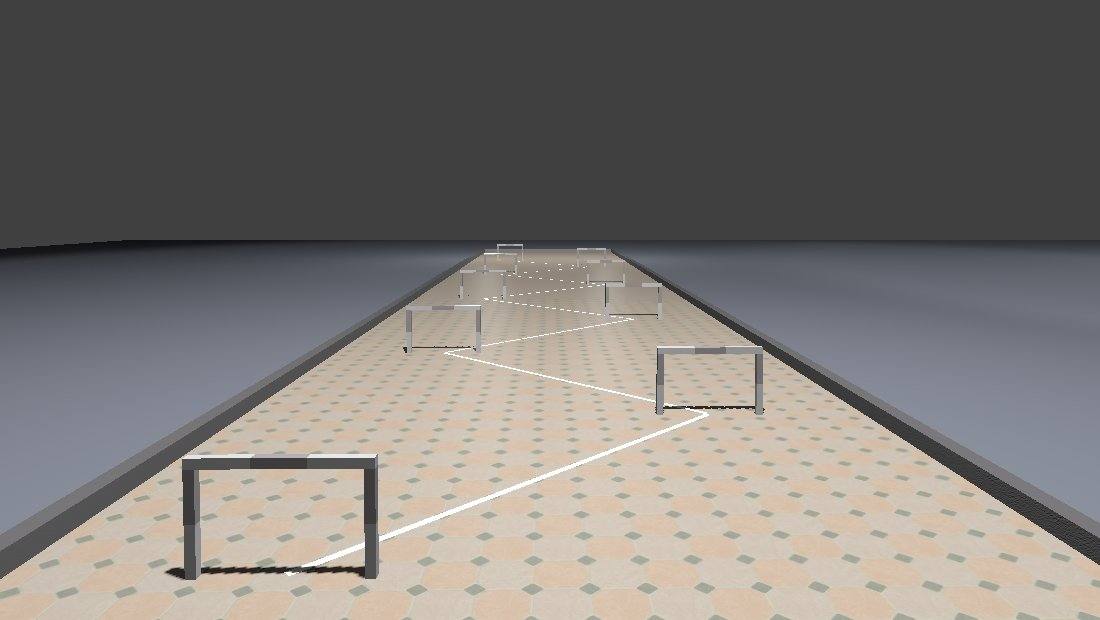
\includegraphics[width=0.8\textwidth]{figures/ch3/t1}
  \caption{\label{fig:3_task1}A screen-shot of the virtual scene used in Experiment T.}
\end{figure}

\paragraph{Results}
We first tested the effects on two independent variables: the translation gain function (linear or divergent) and neutral position type (fixed or adaptive). Then to see interaction effects between these two variables, we further compared the four navigation techniques.

\begin{table*}[!t]
\renewcommand{\arraystretch}{1.3}
\caption{Results of Experiment T}
\label{tab:3_result_t1}
\centering
\begin{tabular}{l l l l}
  \hline
  Variable & Gain Function Type & Neutral Position Type & Technique T1 $\sim$ T4 \\
  \hline
  Time & Divergent\textless Linear & / & T1\textgreater \{T3, T4\}; T2\textgreater T4 \\
  Length & / & / & / \\
  Hazardous Area Consumption & Divergent\textless Linear & / & T1\textgreater \{T3, T4\}; \\
  Shared Workspace Occupation & Divergent\textless Linear & / & T1\textgreater T4; T1\textgreater T3 (0.054); T2\textgreater T4 (0.055) \\
  \hline
\end{tabular}
\end{table*}

Results showed that the gain function type had a significant influence on multiple dependent variables while the neutral position type did not (Table~\ref{tab:3_result_t1}). For navigation time, divergent gain function (mean=89.5, sd=17.8) was faster than the linear one (mean=113.0, sd=21.1) (F(1, 46)=17.25, p\textless 0.001). For Hazardous Area Consumption, divergent gain function (mean=111.57, sd=15.17) had lower score than the linear one (mean=132.58, sd=22.22) (F(1, 46)=14.63, p\textless 0.001). Same for Shared Workspace Occupation, divergent gain function (mean=5.18, sd=3.26) had lower score than the linear one (mean=12.58, sd=8.99) (F(1, 46)=14.38, p\textless 0.001).


\subsubsection{Experiment R}
\paragraph{Design}
We compared the four navigation techniques in the second group (R1 - R4) which only allowed rotations. We asked participants to turn each time virtually 180 degrees to perform an object picking task. Each navigation technique was tested once and the four conditions were randomized for different groups of participants.

The task was to pick up an object behind a user and put it into the orange cube on the table in front (Figure~\ref{fig:3_task2}). Participants were asked to stay on the neutral position and to keep their feet fixed on the floor since we did not want to involve translation. As a consequence, in this experiment we could only test a specific value of adaptive neutral orientation (the bissectrice of rotational workspace) compared to an empirically chosen direction (facing front screen).

We used green arrows to indicate the right rotation direction for the participants so overall they had equal left and right rotations.

\paragraph{Results}
We first tested the effects on two independent variables: the rotation gain function (linear or saturated quadratic) and neutral orientation type (face front screen or bissectrice). Then to see interaction effects between these two variables, we further compared the four navigation techniques.

\begin{figure}[tb]
  \centering
  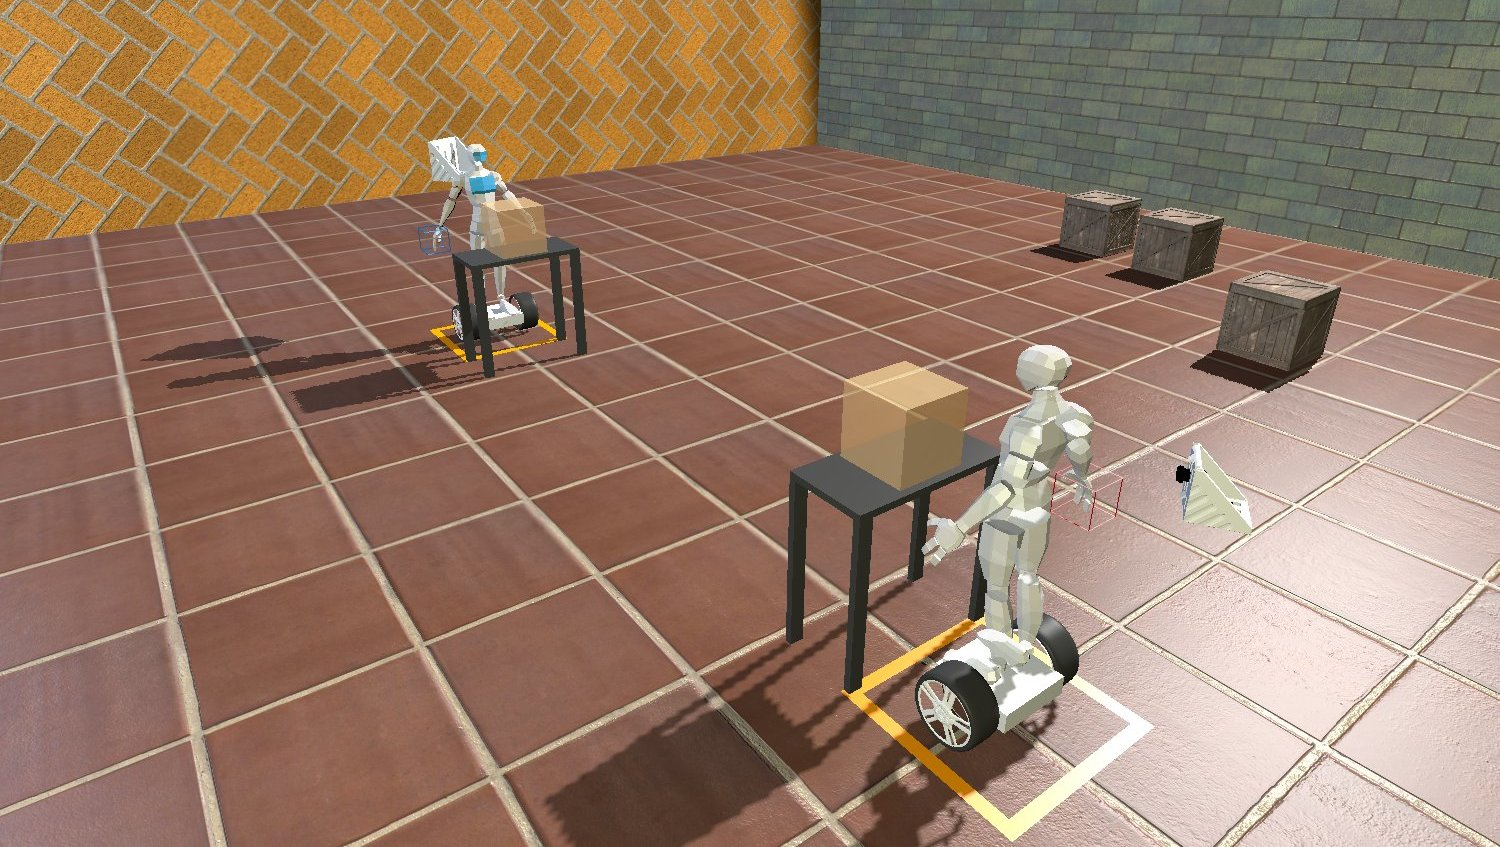
\includegraphics[width=0.8\textwidth]{figures/ch3/t2}
  \caption{\label{fig:3_task2}A screen-shot of the virtual scene used in Experiment R.}
\end{figure}

\begin{table*}[!t]
\renewcommand{\arraystretch}{1.3}
\caption{Results of Experiment R}
\label{tab:3_result_t2}
\centering
\begin{tabular}{l l l l}
  \hline
  Variable & Gain Function Type & Neutral Orientation Type & Technique R1 $\sim$ R4 \\
  \hline
  Time & Saturated quadratic\textless Linear & / & R2\textgreater \{R3, R4\} \\
  Empty Screen Perception & Saturated quadratic\textless Linear & / & \{R1, R2\}\textgreater\{R3, R4\} \\
  User Occlusion & Saturated quadratic\textless Linear & / & R1\textgreater R3 (0.076), R1\textgreater R4 (0.053); R2\textgreater \{R3, R4\} \\
  \hline
\end{tabular}
\end{table*}

Results showed that the gain function type had a significant influence on multiple dependent variables while the neutral orientation type did not (Table~\ref{tab:3_result_t2}). For task finish time, saturated quadratic gain function (mean=13.6, sd=5.0) was faster than the linear one (mean=27.6, sd=15.9) (F(1, 46)=17.09, p\textless 0.001). For Empty Screen Perception, saturated quadratic gain function (mean=59.57, sd=34.61) had lower score than the linear one (mean=196.21, sd=92.06) (F(1, 46)=46.32, p\textless 0.001). For User Occlusion, saturated quadratic gain function (mean=66.69, sd=51.69) also had lower score than the linear one (mean=264.82, sd=219.62) (F(1, 46)=18.51, p\textless 0.001).


\subsubsection{Experiment TR}

\paragraph{Design}
This last experiment aimed to evaluate the 3DoF version human joystick with full translation and rotation control. We compared the eight navigation techniques in the third group (TR1 - TR8), we asked participants to perform a navigation task several times with each time a different technique. Each navigation technique was tested once and the eight conditions were randomized for different groups of participants.

Similar to Experiment T, the task was to travel to the other end of an ``S" shaped corridor by following a given path marked by a white line on the floor and crossing all the gates along the path (Figure~\ref{fig:3_task3}). Each pair of participants had symmetric path to walk through and they were free to use translation combined with rotation.

To begin, participants left their departure areas and traveled to destination zones on the other side of the corridors. Once both participants arrived, they were transported to a separated virtual space to finish the aforementioned cohabitation questionnaire by selecting a response with a tracker on the right hand (Figure~\ref{fig:3_task3_q}). There were six answer levels from negative to positive answers represented by six floating cubes from left to right. For example, the leftmost one meant ``I do not agree at all" and the rightmost ``I totally agree", etc.  When both participants finished all the seven questions, they were transported again to the departure areas to begin the next round with a different navigation technique till all the conditions were tested.

\begin{figure}[tb]
  \centering
  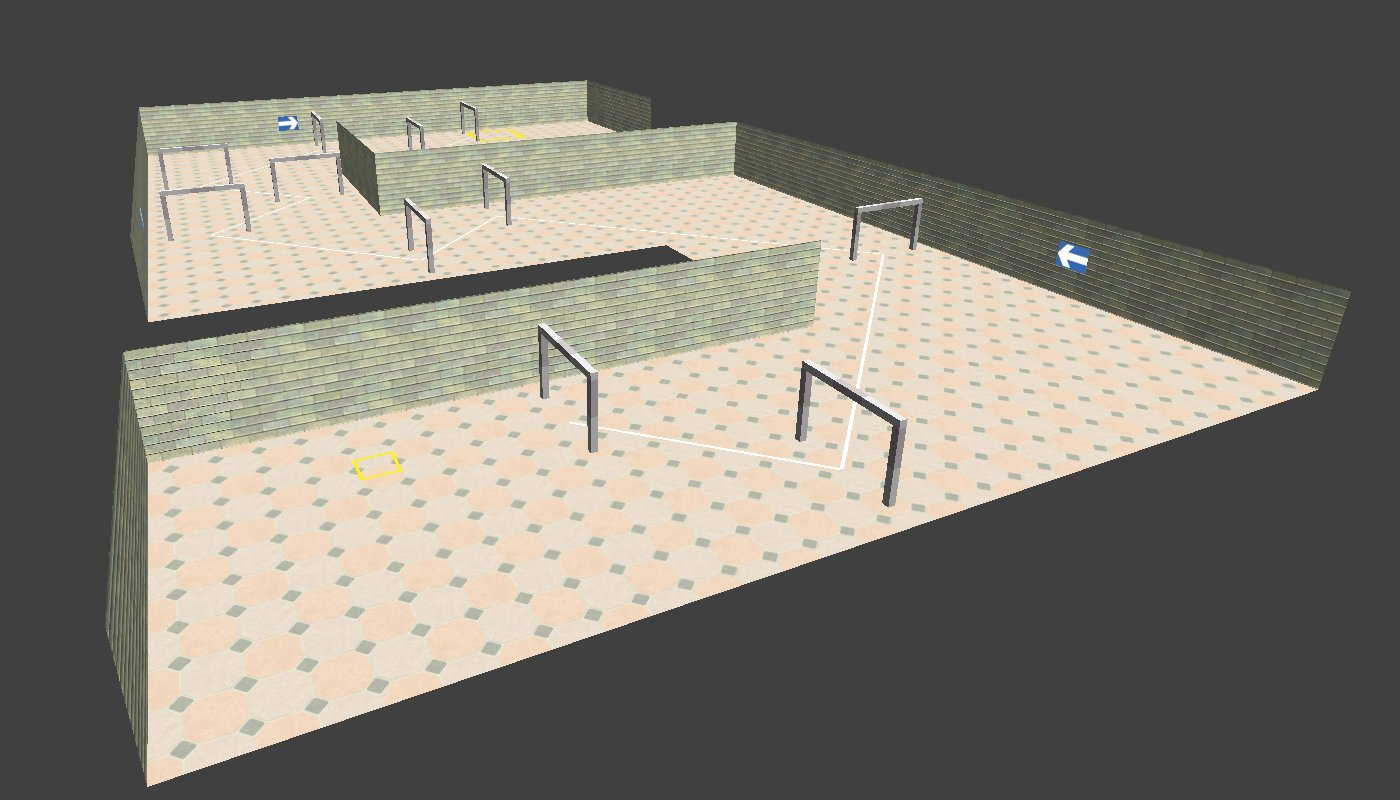
\includegraphics[width=0.8\textwidth]{figures/ch3/t3}
  \caption{\label{fig:3_task3}A screen-shot of the virtual scene used in Experiment TR.}
\end{figure}

\begin{figure}[tb]
  \centering
  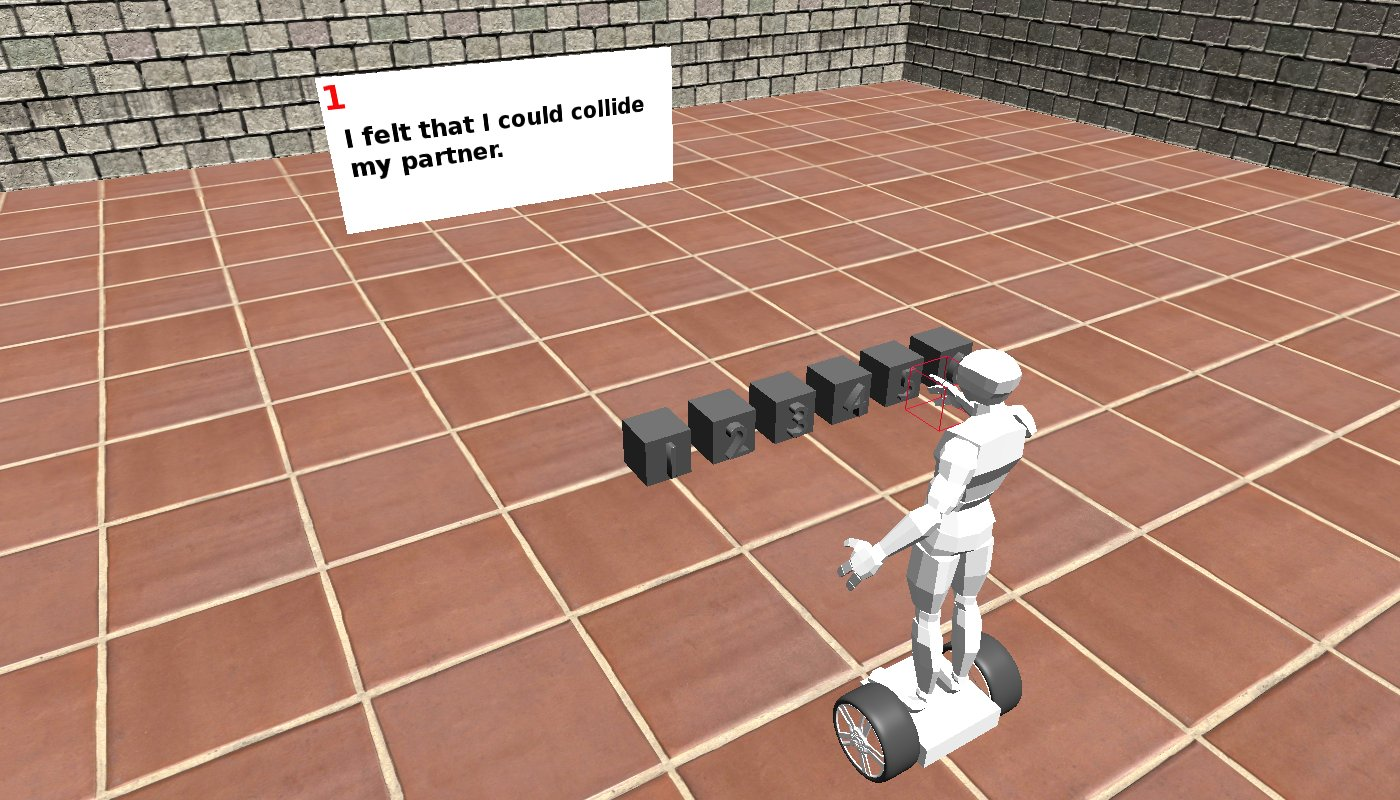
\includegraphics[width=0.8\textwidth]{figures/ch3/t3_q}
  \caption{\label{fig:3_task3_q}Participants filled a questionnaire about user cohabitation presented on a virtual screen.}
\end{figure}


\paragraph{Results}
We first tested the effects on three independent variables: the gain function type (linear or modified), neutral position and neutral orientation types (fixed or adaptive). Then to see interaction effects between these variables, we further compared the eight navigation techniques.

\begin{table*}[!t]
\renewcommand{\arraystretch}{1.5}
\caption{Results of Experiment TR}
\label{tab:3_result_t3}
\centering
\begin{tabular}{p{1.6cm} | p{1.8cm} p{2.2cm} p{2cm} p{2.2cm} p{5.8cm}}
  \hline
   & Variable & Gain Function Type & Neutral Position Type & Neutral Orientation Type & Technique TR1 $\sim$ TR8 \\
  \hline
  Navigation Performance & Time & Modified\textless Linear & / & / & \{TR1, TR2, TR3, TR4\}\textgreater \{TR5, TR6, TR7, TR8\} \\
  \cline{2-6}
   & Length & Modified\textless Linear & / & / & TR3\textgreater \{TR5, TR6, TR7\}; TR4\textgreater TR7; TR2\textgreater TR7 (0.052); TR4\textgreater TR5 (0.06) \\ \hline \hline
   & Hazardous Area Consumption & Modified\textless Linear & / & / & \{TR1, TR2, TR3, TR4\}\textgreater \{TR5, TR6, TR7, TR8\} \\
   \cline{2-6}
  Cohabitation Capacity & Shared Workspace Occupation & Modified\textless Linear & Adaptive\textless Fixed (p=0.1) & / & \textbf{TR1}\textgreater \{\textbf{TR4}, TR5, TR6, TR7, TR8\}; \newline \{TR2, TR3\}\textgreater \{TR5, TR6, TR7, TR8\} \\
  \cline{2-6}
   & Empty Screen Perception & Modified\textless Linear & / & Fixed\textless Adaptive & \textbf{TR1}\textless \{\textbf{TR2, TR4}\}; \textbf{TR3\textless TR4} \newline \{TR2, TR4\}\textgreater \{TR5, TR6, TR7, TR8\};  \\
   \cline{2-6}
   & User Occlusion & Modified\textless Linear & / & Adaptive\textless Fixed & \textbf{TR1}\textgreater \{\textbf{TR2, TR4}, TR5, TR6, TR7, TR8\}; TR2\textgreater \{TR6, TR7, TR8\}; \textbf{TR3}\textgreater \{\textbf{TR2, TR4}, TR5, TR6, TR7, TR8\}; TR4\textgreater \{TR6, TR7, TR8\}; \\ \hline \hline
   & Question 1 & Modified\textless Linear & / & / & TR1\textgreater \{TR5, TR6, TR7, TR8\}; TR4\textgreater TR6 (0.054) \\
   \cline{2-6}
   & Question 2 & Modified\textless Linear & / & / & \{TR1, TR4\}\textgreater \{TR5, TR6, TR7, TR8\} \\
   \cline{2-6}
   & Question 3 & Modified\textless Linear & / & / & \{TR1, TR3, TR4\}\textgreater \{TR5, TR6, TR7, TR8\} \\
   \cline{2-6}
  Questionnaire & Question 4 & Modified\textless Linear & / & / & \{TR1, TR2, TR3, TR4\}\textgreater \{TR5, TR6, TR7, TR8\} \\
  \cline{2-6}
   & Question 5 & Modified\textless Linear & / & / & TR1\textgreater \{TR5, TR6, TR7, TR8\}; TR2\textgreater TR5; TR3\textgreater TR5; TR3\textgreater \{TR6, TR7, TR8\} (0.065); TR4\textgreater TR5 (0.065) \\ \cline{2-6}
   & Question 6 & Modified\textless Linear & / & / & \{TR1, TR3, TR4\}\textgreater \{TR5, TR6, TR7, TR8\} \\ \cline{2-6}
   & Question 7 & Modified\textless Linear & / & / & \{TR1, TR3\}\textgreater \{TR5, TR6, TR7, TR8\}; TR4\textgreater TR6 \\
  \hline
\end{tabular}
\end{table*}

Results showed that the gain function type had a significant influence on multiple dependent variables. Modified gain functions (divergent for translation, saturated quadratic for rotation) tended to provide better navigation efficiency and improved cohabitation capacity (Table~\ref{tab:3_result_t3}). Figure~\ref{fig:3_exp_tr_box} showed a detailed view of results on cohabitation measurements grouped by navigation techniques.

\begin{figure*}[tb]
  \centering
  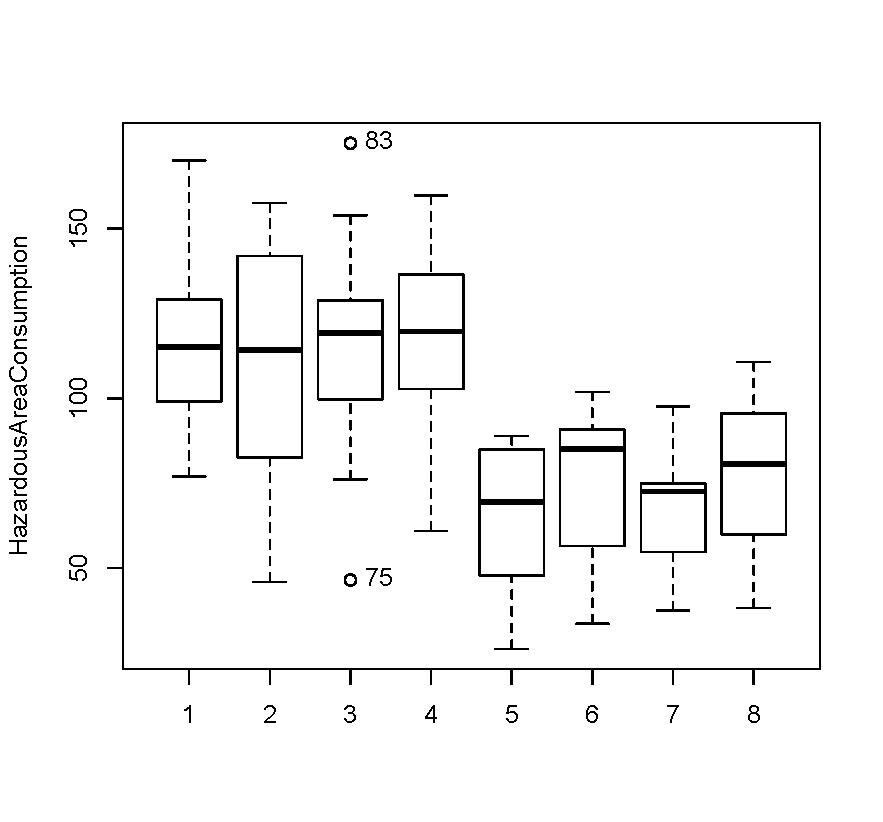
\includegraphics[width=0.48\textwidth]{figures/ch3/HAC}
  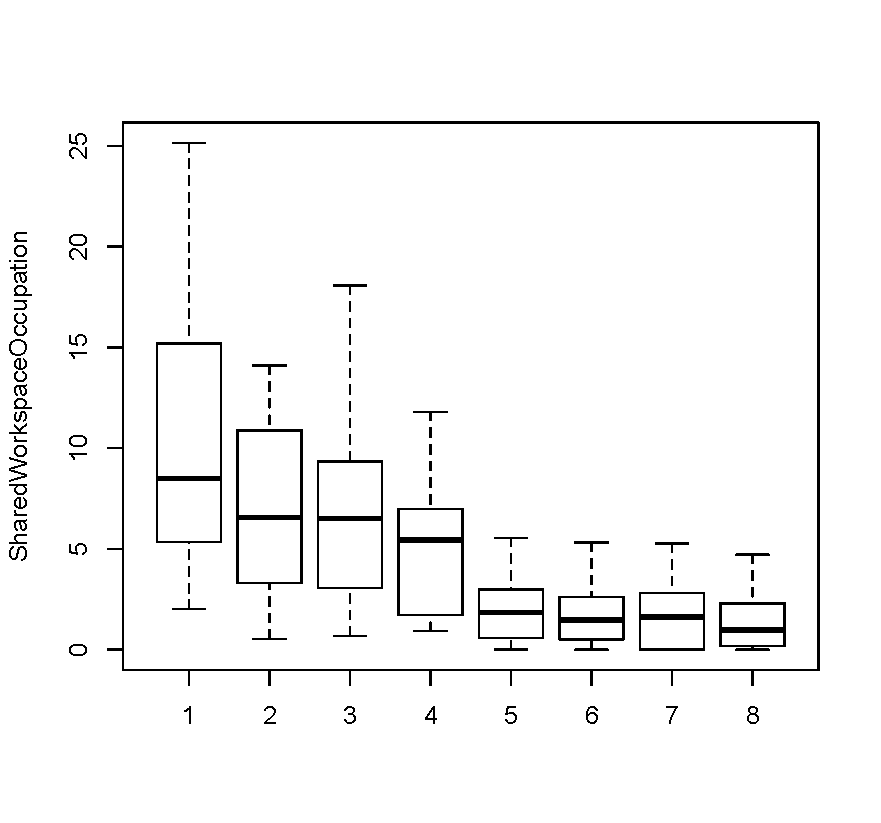
\includegraphics[width=0.48\textwidth]{figures/ch3/SWO}
  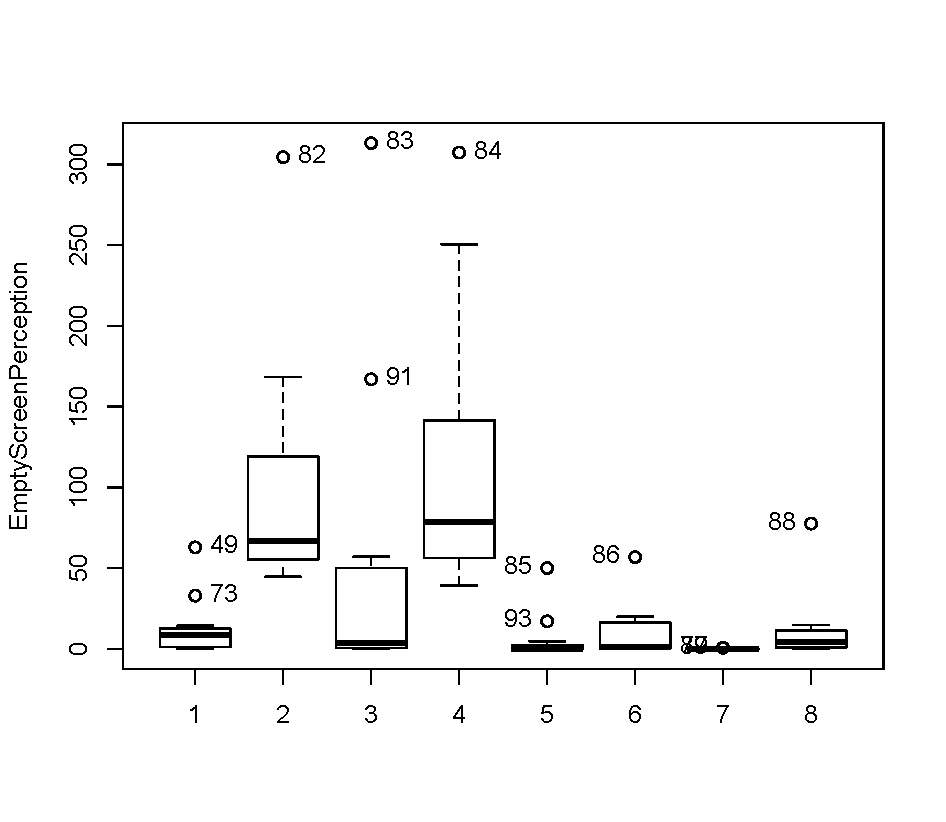
\includegraphics[width=0.48\textwidth]{figures/ch3/ESP}
  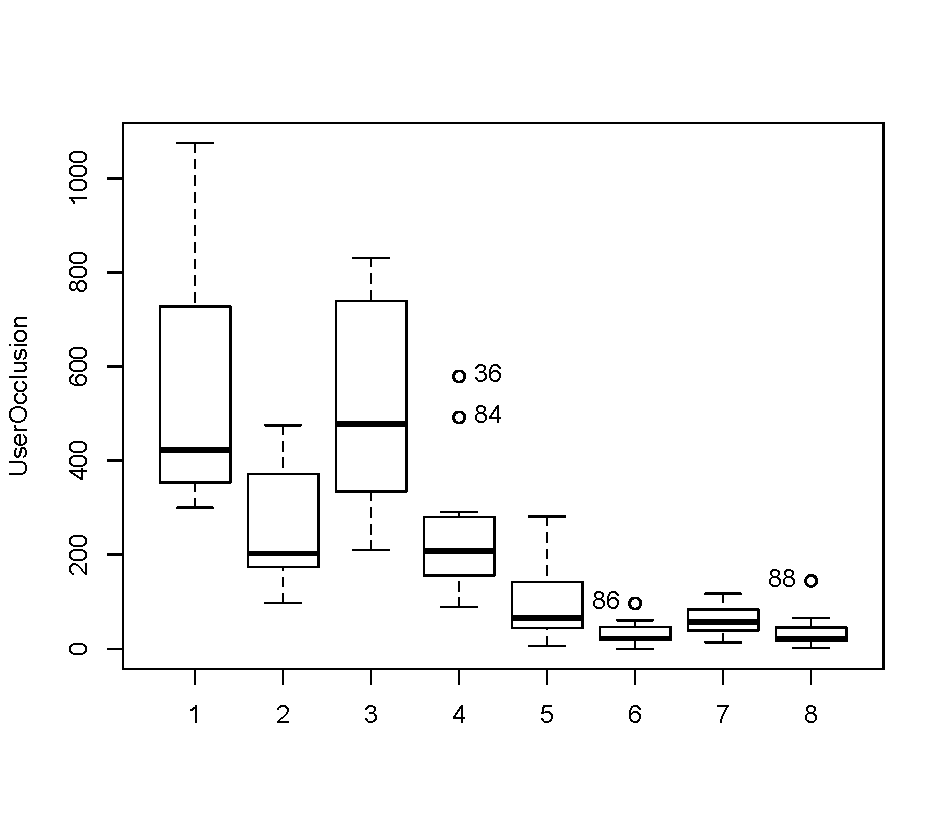
\includegraphics[width=0.48\textwidth]{figures/ch3/UO}
  \caption{\label{fig:3_exp_tr_box}Boxplot for conditions from TR1 to TR8 (marked as 1 to 8) on cohabitation measurements in Experiemnt TR. The numbers in the graph are outlier observations.}
\end{figure*}

Modified gain function (mean=67.1, sd=13.8) was faster than the linear one (mean=101.2, sd=14.8) (F(1, 94)=136.6, p\textless 0.001), and had a shorter path (mean=100.51, sd=2.41) than the linear one (mean=104.21, sd=4.46) (F(1, 94)=25.45, p\textless 0.001), knowing that the optimal path was 98 meters long (marked by white line on the floor in Figure~\ref{fig:3_task3}). For Hazardous Area Consumption, modified gain function (mean=71.59, sd=20.77) had lower score than the linear one (mean=114.86, sd=29.82) (F(1, 94)=68.05, p\textless 0.001). For Shared Workspace Occupation, modified gain function (mean=1.71, sd=1.57) also had lower score than the linear one (mean=7.50, sd=5.60) (F(1, 94)=47.5, p\textless 0.001). Concerning rotational aspects, for Empty Screen Perception, modified gain function (mean=6.83, sd=15.53) had lower score than the linear one (mean=68.78, sd=83.08) (F(1, 94)=25.79, p\textless 0.001). For User Occlusion, modified gain function (mean=55.69, sd=52.57) also had lower score than the linear one (mean=393.58, sd=233.79) (F(1, 94)=95.44, p\textless 0.001).

The type of neutral reference frame did not seem to influence navigation efficiency, however, we observed some effects on cohabitation capacity. For Empty Screen Perception, fixed neutral orientation (mean=17.14, sd=51.65) had lower score than the adaptive one (mean=58.46, sd=74.59) (F(1, 94)=9.957, p=0.00215). However, fixed neutral orientation (mean=304.09, sd=284.59) had higher score than the adaptive one (mean=145.18, sd=147.77) for User Occlusion (F(1, 94)=11.79, p\textless 0.001). In addition, neutral position type tended to have an effect on Shared Workspace Occupation (trend effect): adaptive neutral position (mean=3.76, sd=3.89) had lower score than the fixed one (mean=5.45, sd=5.86) (F(1, 94)=2.76, p=0.1).

Regarding the cohabitation questionnaire, we got similar results from question 1 to question 7: modified gain functions globally had lower scores than linear gain functions, whereas neutral reference frame type did have significant influence on users' subjective feeling towards user cohabitation (Figure~\ref{fig:3_questionnaire}).

\begin{figure*}[tb]
  \centering
  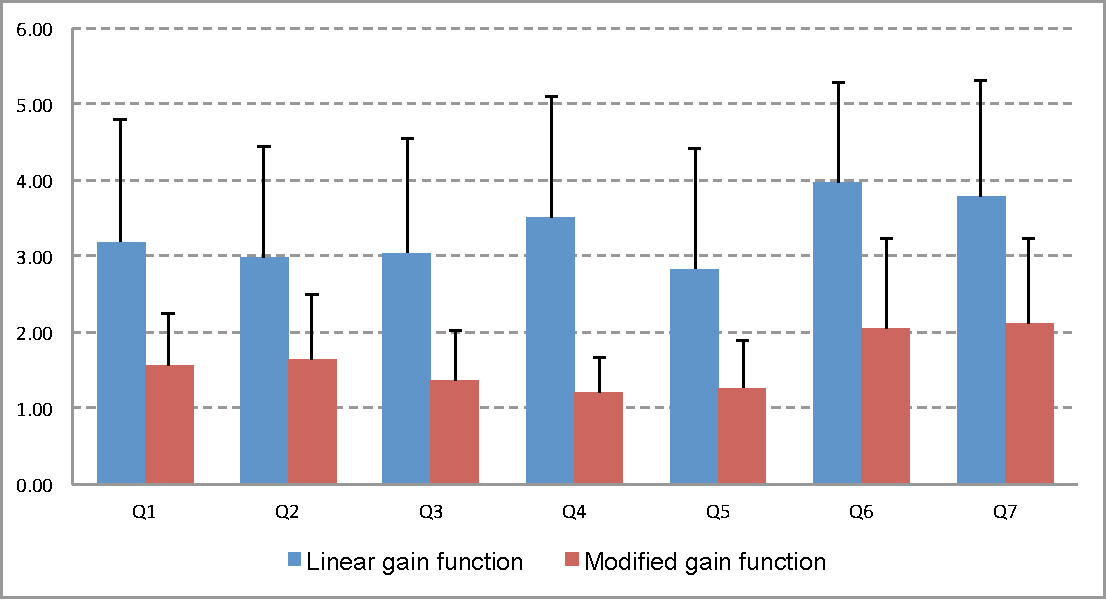
\includegraphics[width=0.53\textwidth]{figures/ch3/qn_bar}
  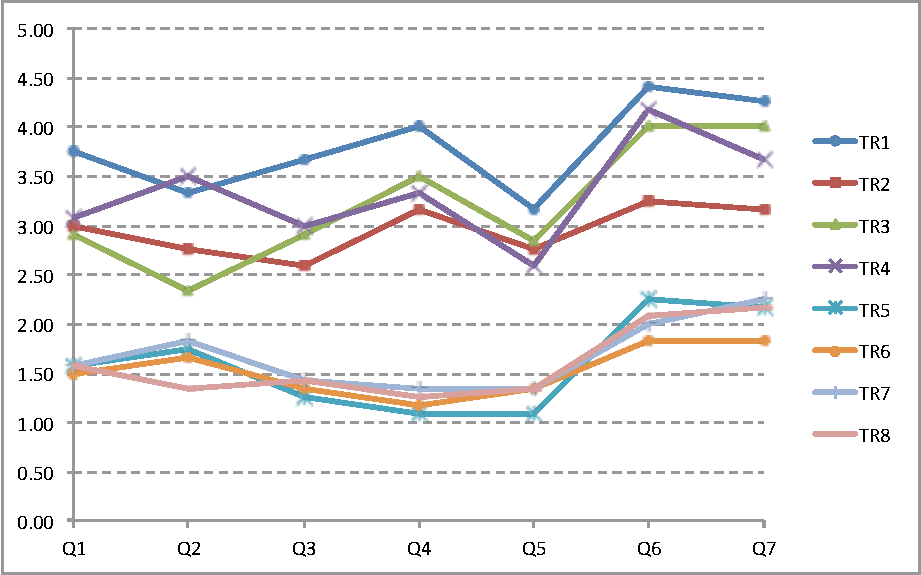
\includegraphics[width=0.46\textwidth]{figures/ch3/qn_line}
  \caption{\label{fig:3_questionnaire}Cohabitation questionnaire scores grouped by gain function type (left) and by navigation condition (right).}
\end{figure*}

\subsubsection{Discussion}
From the above three experiments, we could clearly see that modified gain functions had a significant influence on users' navigation efficiency and cohabitation capacity, shown by both objective and subjective measurements. The divergent and quadratic gain functions allowed users to get a much higher navigation speed before reaching the borders of the physical workspace. As discussed in previous experiment, linear gain functions with higher gain value could also reduce cohabitation problems, but at a cost on low speed control precision, which can be observed from difference of trajectory lengths in Experiment TR. So in general, the modified gain functions, which take the border of physical workspace into consideration for velocity computation, are more suitable than linear gain functions to ensure safe navigation in restricted physical workspace with human joystick metaphor.

We could also see that in Experiment TR, adaptive neutral orientation reduced user occlusion, same as we found in previous experiment, though we were not able to confirm this effect in Experiment R (rotation only test) since users did not change their positions. However, on the other hand, adaptive neutral orientation led to more empty screen perception, which was not observed in previous experiment. In fact, as shown by Figure~\ref{fig:3_neutral_ref}, adaptive neutral orientation provides a compromised solution between two kinds of constrains, the empty screen and the other user, and it is normal that moving the neutral orientation away from the other user will result in more empty screen perception.

Overall, if we combine these two rotation-related variables into a new one representing user's perception of real world, techniques with adaptive neutral orientation (mean=62.51, sd=61.49) still had much lower total score than those having fixed neutral orientations (mean=462.36, sd=241.03) (p \textless{} 0.001). So using adaptive neutral orientation with modified gain functions could globally lower the perception of physical environment.

Although we had expected similar benefits from adaptive neutral position as we got by changing neutral orientations, we did not get any effect on measurements used in Experiment T, and only got a trend effect (p = 0.1) on shared workspace occupation.

A closer look on the effects of adaptive neutral reference frames showed that, significant differences lay only between techniques with linear gain functions (bold part in Table~\ref{tab:3_result_t3} and Figure~\ref{fig:3_exp_tr_box}). The modified gain functions largely compensated cohabitation problem no matter the type of neutral orientation and position. Despite the fact that we did not find significant differences between techniques with modified gain functions (from TR5 to TR8), we could still get some observations from Figure~\ref{fig:3_exp_tr_box}: first, the results of linear gain group (TR1 to TR4) and modified gain group (TR5 to TR8) seemed to have the same distribution, though the fluctuation was in a much smaller scale for modified gain group, which meant the adaptive neutral frames did have an impact on conditions in the modified gain group, but not enough to be observable; second, TR8 was not always the technique that provided best cohabitation capacity, so it might not be a good idea to change the neutral position and orientation simultaneously, or it should be done in a more intelligent way.

Regarding the questionnaire of cohabitation, we almost got the same result with objective measurements: two clusters of techniques were clearly identified - techniques with linear gain functions nearly doubled the scores on all the questions (Figure~\ref{fig:3_questionnaire}). However, participants were not able to feel the influence of adaptive neutral reference frames, whose effects may be covered by the significant improvements brought by modified gain functions. Another test with merely modified gain functions should be added if we want to further compare different types of neutral reference frames with subjective measurements.

\subsection{Summary}
In this paper we presented several modifications of the human joystick metaphor in order to enable individual navigation for co-located users in a multi-stereoscopic immersive virtual environment and to solve associated cohabitation problems. The alterations were designed to help users avoid physical obstacles and non-usable part of the display by directly integrating limitations of the physical system and the influence of other users into the paradigm, so to assure users' safety and level of immersion. Then we summarized an evaluation model to assess user cohabitation capability, using different variables to quantify the risk of collision and perceptual disturbance.

We conducted a series of user evaluations to investigate the influence of each alteration by testing their combinations with various navigation tasks. Results showed that modified gain functions could provide a larger velocity range with relatively small base gain value compared to linear gain functions, thus could largely improve users' cohabitation situation both for translation and rotation. Adaptive neutral orientations can efficiently reduce user occlusion, more generally user's perception of physical environment. Whereas adaptive neutral positions only showed some potential benefits and needed to be further developed. For example, the optimal distribution of the neutral positions is not necessarily the median of each user's workspace, but can be more flexible depending on both users' activities in real time (velocity in physical workspace, navigation strategy, etc.).

Finally, in spite of our work to propose measurements which characterize efficiently navigation performance as well as user cohabitation, some limitations remain to be solved. For example, a user staying for a very long time in the peripheral field of view of another user may not be as disturbing as a user standing right in front of another for a few seconds even though the latter has a lower occlusion score.

\section{Conclusion}


